\chapter
\section{Beschleunigermagnet, FEMM}

In Abbildung \ref{fig:Linear} ist der Verlauf des Magnetfeldes in einem vereinfachten Modell des Beschleunigermagnets SIS-100, der im FAIR Projekt der Gesellschaft für Schwerionenforschung verwendet wird, zu sehen. In dieser Simulation wurde ein linearer Materialzusammenhang zwischen magnetischer Flussdichte B und magnetischer Feldstärke H angenommen. Das B-Feld hat hierbei ein Maximum von ca. $\SI{5,7}{Tesla}$. Die Flusslinien sind annähernd homogen allerdings ist zu erkennen, dass in der Nähe des Luftspaltes die Flusslinien deutlich näher beieinander liegen.

\begin{figure}[h!]
	\centering
	\begin{subfigure}[h]{.28\textwidth}
		\centering
		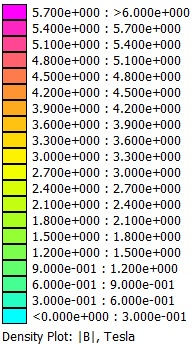
\includegraphics[width=\textwidth]{data/skala_linear}
		\caption{Skala}
		\label{fig:SkalaLin}
	\end{subfigure}
	\begin{subfigure}[h]{.60\textwidth}
		\centering
		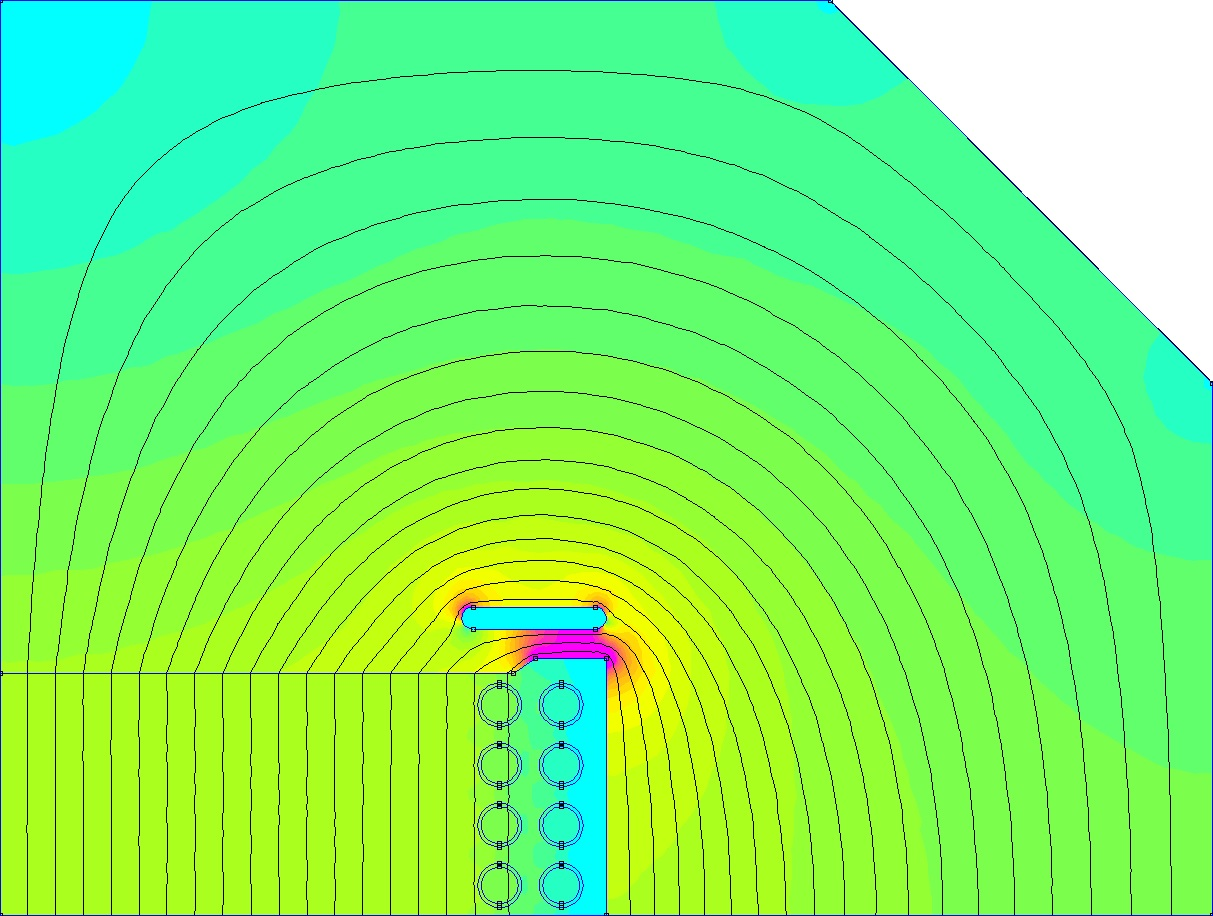
\includegraphics[width=\textwidth]{data/Linear}
		\caption{Lineare statische Simulation des Beschleunigermagnets SIS-100 in FEMM}
		\label{fig:Linear}
	\end{subfigure}	
\end{figure}

Weist man dem Eisenjoch eine nichtlineare Materialbeziehung zu ergibt sich daraus Abbildung \ref{fig:NichtLinear}. Der maximale Wert des B-Felds ist hier mit ca. $\SI{2,1}{Tesla}$ geringer als bei der linearen Simulation. Außerdem sind die Flusslinien noch deutlich homogener verteilt. Das liegt daran, dass bei dieser Simulation das Eisenjoch in Sättigung geht.

\begin{figure}[h!]
	\centering
	\begin{subfigure}[h]{.28\textwidth}
		\centering
		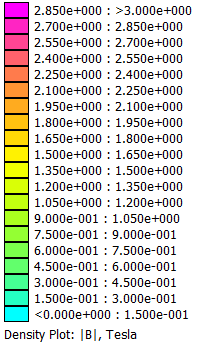
\includegraphics[width=\textwidth]{data/Skala_nichtlinear}
		\caption{Skala}
		\label{fig:SkalaNonlin}
	\end{subfigure}
	\begin{subfigure}[h]{.60\textwidth}
		\centering
		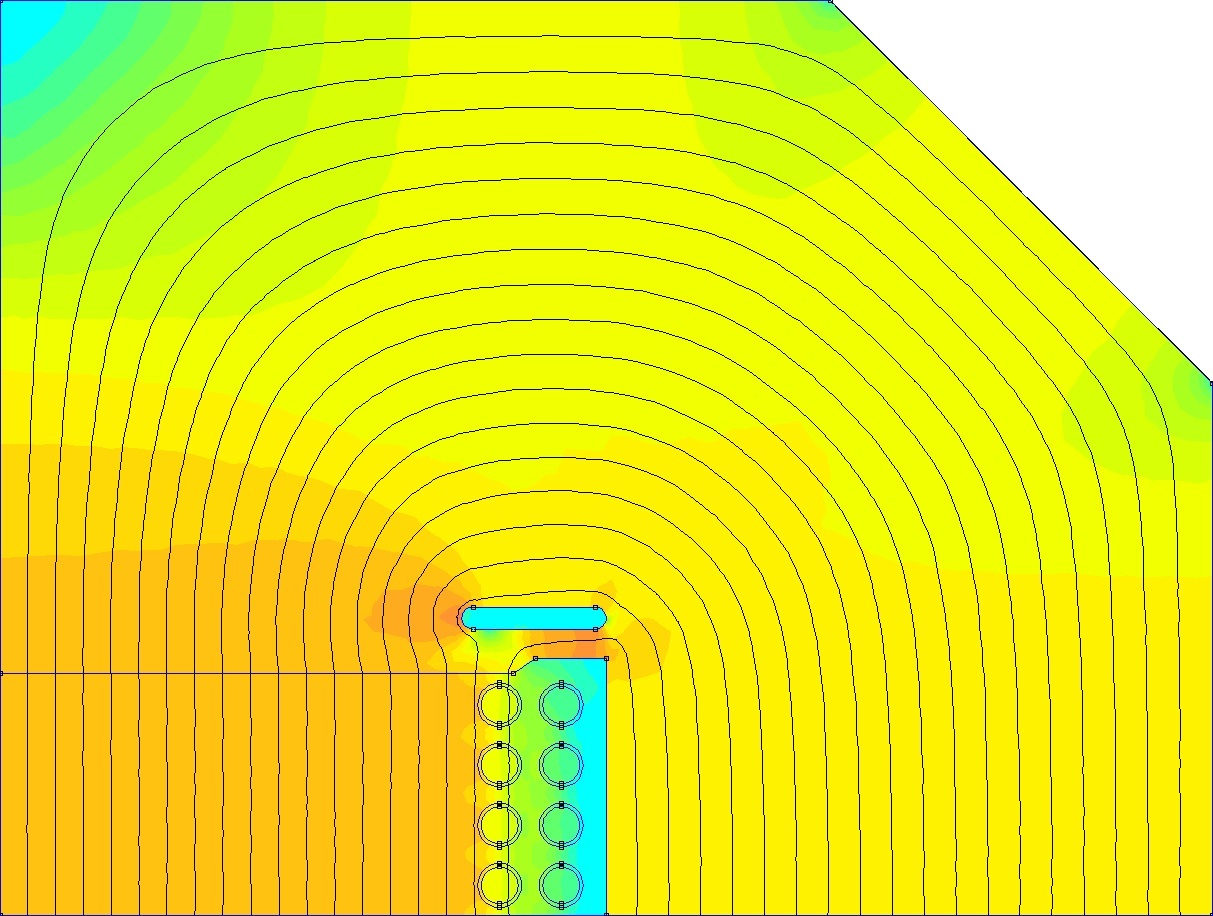
\includegraphics[width=\textwidth]{data/Nichtlinear}
		\caption{Simulation des Beschleunigermagnets SIS-100 mit nichtlinearer Materialbeziehung}
		\label{fig:NichtLinear}
	\end{subfigure}	
\end{figure}

Über die Funktion \texttt{lineintegral} lässt sich die durchschnittliche Flussdichte über einen bestimmten Bereich berechnen. Mit 

\begin{equation*}
	L = \frac{\Psi}{I}
\end{equation*}

und

\begin{equation*}
	\Psi = \int_{A} \vec{B} \mathrm{d}\vec{A}
\end{equation*}

ergibt sich die Induktivität zu

\begin{equation*}
	L = \frac{B A}{I}
\end{equation*}
 

 Wie in Abbildung \ref{fig:plot} zu sehen ist, nimmt die Induktivität kontinuierlich ab, sobald eine Stromanregung von etwa $\SI{6000}{A}$ angelegt wird da dann der Eisenkern in Sättigung geht.


\begin{figure}[h]
	\centering
	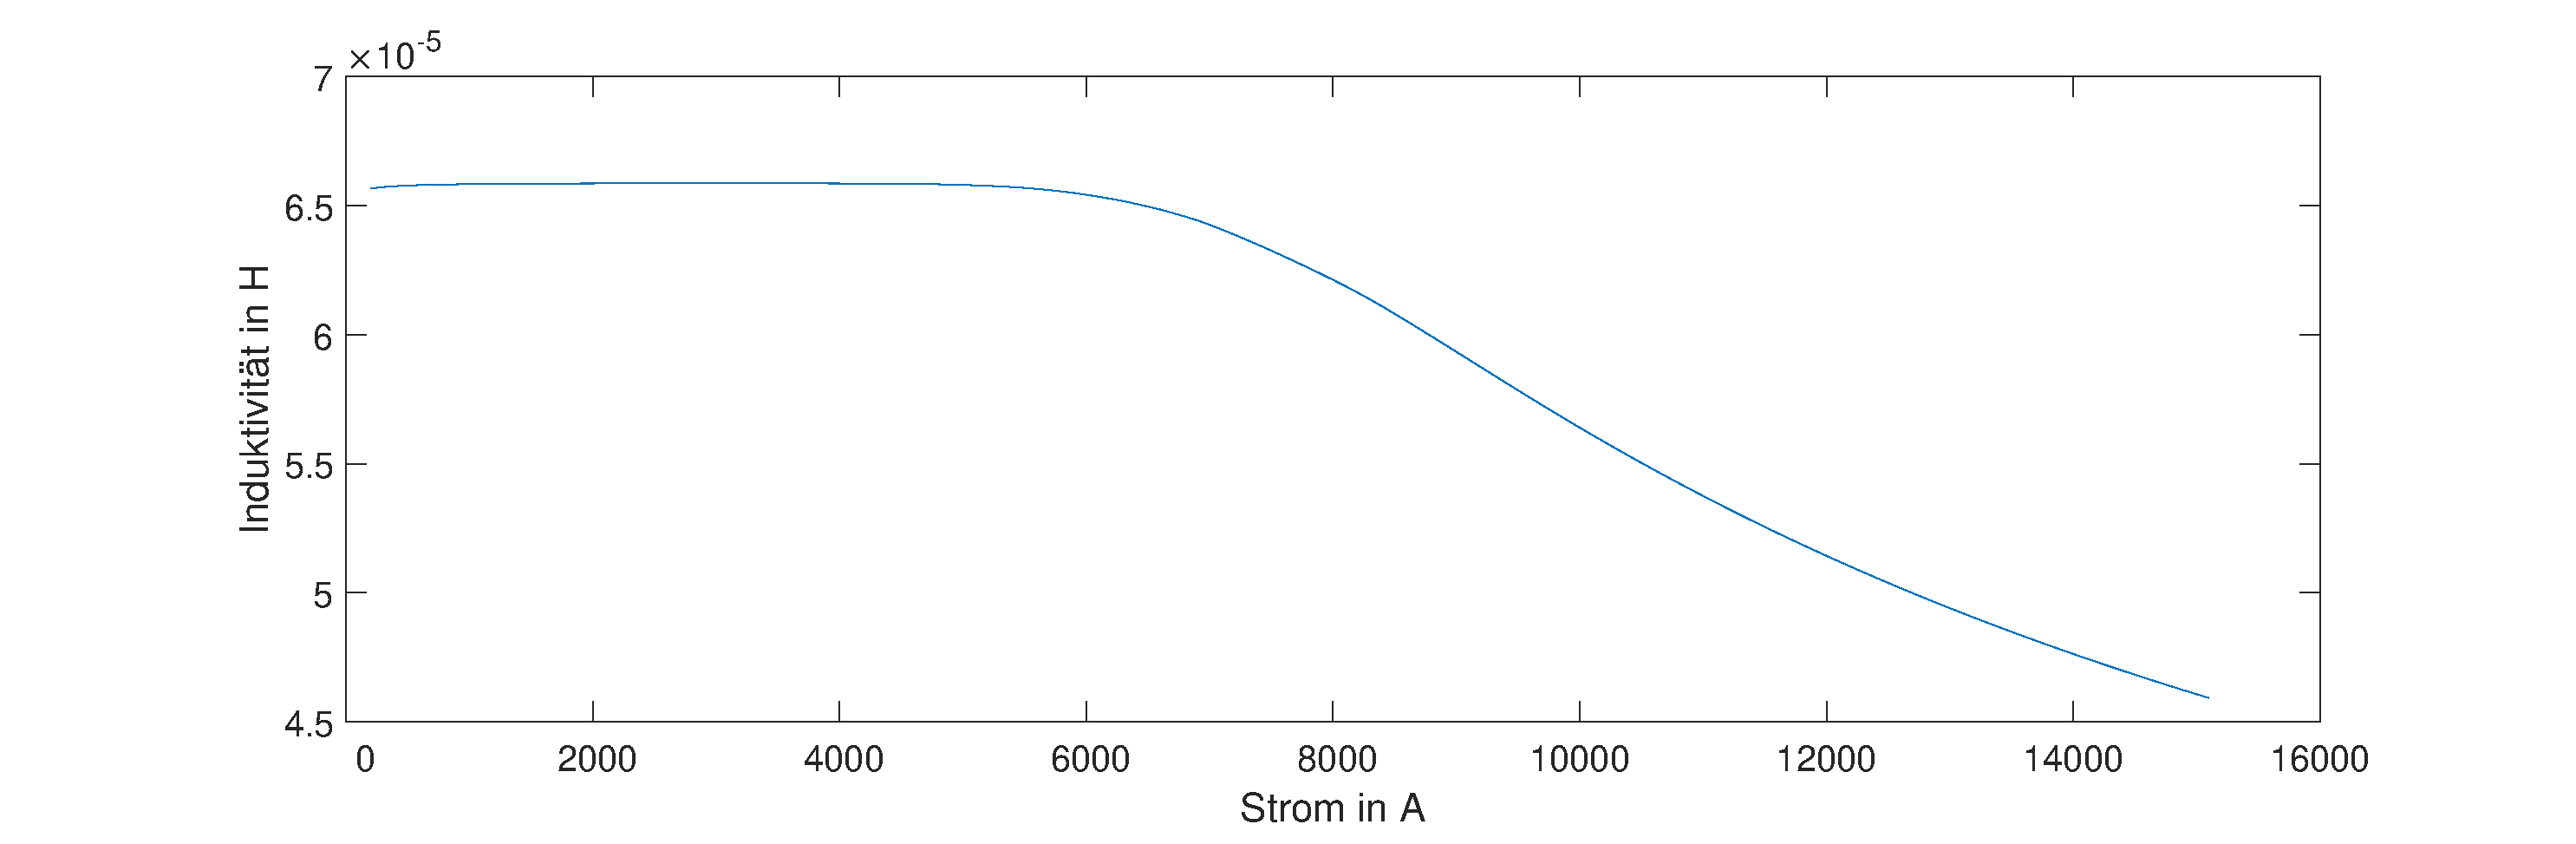
\includegraphics[width=\textwidth]{data/Ag8_3dplot}
	\caption{Induktivität in Abhängigkeit der Stromanregung}
	\label{fig:plot}
\end{figure}